\section{Architettura del prodotto}

\subsection{Descrizione generale}

Il gruppo \Omicron{} ha deciso di modellare l'architettura del prodotto in due moduli distinti:
\begin{itemize}
\item \textbf{Front-end}: modulo che gestisce l'interfaccia grafica e l'interazione diretta con gli utenti;
\item \textbf{Back-end}: modulo che gestisce la parte relativa al processo dei dati, in particolare dove questi vengono mantenuti e come vengono trattati.
\end{itemize}

La scelta di suddividere il progetto in questi due moduli garantisce un maggiore disaccopiamento fra la parte di \textbf{business logic} e quella di \textbf{presentation logic}. I due moduli interagiscono fra di loro univocamente tramite chiamate API\ped{G}. Tale interazione viene descritta in dettaglio nelle sezioni \S{2.2} e \S{2.3}.

\subsection{Architettura modulo Back-end}


\subsubsection{Descrizione}
In questo modulo, chiamato \textbf{Back-end\ped{G}}, viene gestita la logica interna del sito \nameproject. In particolare viene amministrato l'accesso al lato \textbf{business} dell'applicativo, e la parte relativa alla persistenza dei dati salvati all'interno dei servizi offerti da Amazon AWS\ped{G}. L'architettura generale del modulo è basata sui microservizi offerti dalle chiamate API, i quali hanno una base in comune sviluppata a \textbf{layer}, dove i tre layer principali sono:
\begin{itemize}
	\item \textbf{Handler\ped{G} delle API\ped{G}}: gestori delle richieste suddivise per dominio;
	\item \textbf{Model}: gestione logica dei modelli delle entità rappresentate (prodotto, utente...);
	\item \textbf{Services}: gestione dei servizi Amazon AWS\ped{G} e complementari.
\end{itemize} Il modulo \textbf{Front-end\ped{G}} interagisce con il modulo \textbf{Back-end\ped{G}} attraverso delle chiamate API\ped{G} esposte del servizio Amazon API Gateway. Tali API\ped{G} sono divise per dominio relativo all'oggetto con cui si vuole interagire e alla sua funzionalità (es. inserimento di un nuovo prodotto). L'handler\ped{G} gestisce la richiesta in base alla propria funzionalità e smista la relativa richiesta, dopo un opportuno controllo, sul \textbf{layer dei servizi} (dove necessario). I servizi offerti comprendono l'interfacciamento con DynamoDB, Stripe, S3, Nodemailer, Cognito. Inoltre, sempre dove necessario, l'handler\ped{G} della richiesta può interfacciarsi con il \textbf{layer dei modelli} degli oggetti (prodotto, utente ecc..) i quali forniranno supporto per la gestione logica di tali elementi.

\vspace{1cm}

\begin{figure}[H]
\centering
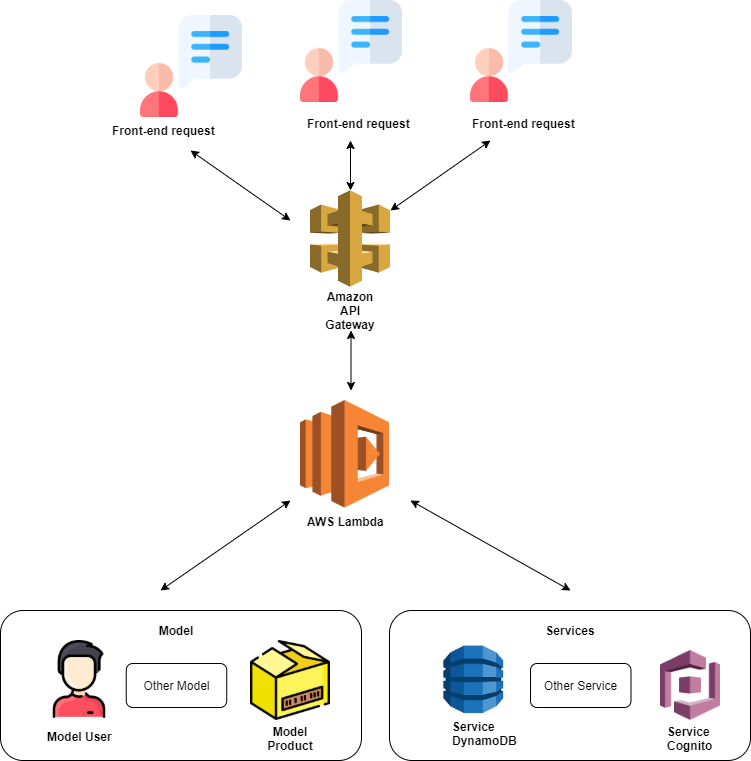
\includegraphics[scale=0.40]{res/Architettura/Backend/img/layerBack-end.png}\\
\caption{Layer del modulo Back-end\ped{G}}
\end{figure}
\subsubsection{Diagramma dei package}

Di seguito è riportato il diagramma dei package\ped{G} del modulo \textbf{Front-end\ped{G}}.

\vspace{1cm}

\begin{figure}[H]
\centering
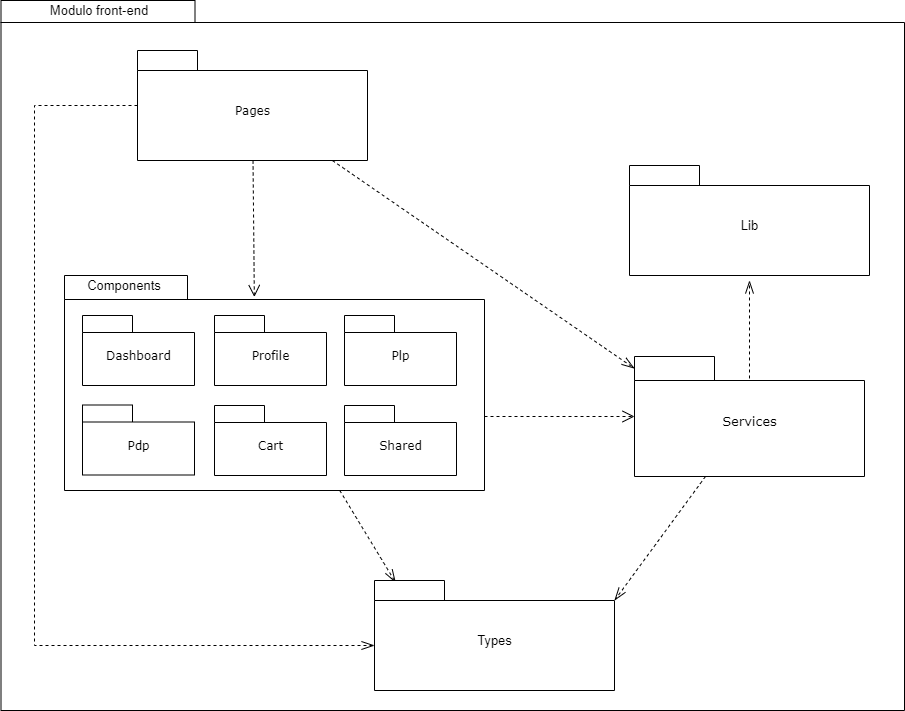
\includegraphics[scale=0.43]{res/Architettura/Frontend/img/package_frontend.png}\\
\caption{Diagramma dei package\ped{G} del modulo Front-end\ped{G}}
\end{figure}
\subsubsection{Diagramma delle classi}
Di seguito è riportato un esempio di diagramma delle classi. Esso rappresenta come è composta la pagina della dashboard\ped{G} e come vengono gestiti i vari component presentational e container.

\vspace{1cm}

\begin{figure}[H]
\centering
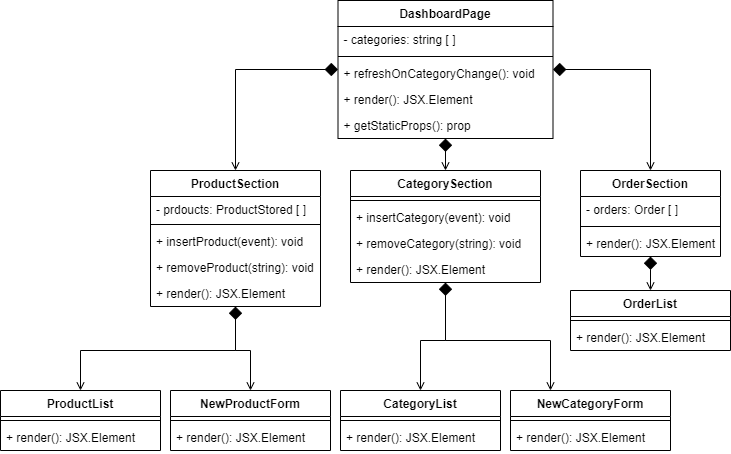
\includegraphics[scale=0.55]{res/Architettura/Frontend/img/class_frontend_dashboard}\\
\caption{Diagramma delle classi della pagina dashboard\ped{G} per il modulo Front-end\ped{G}}
\end{figure}

Viene inoltre mostrato il diagramma per i diversi tipi utilizzati dal nostro modulo.

\begin{figure}[H]
\centering
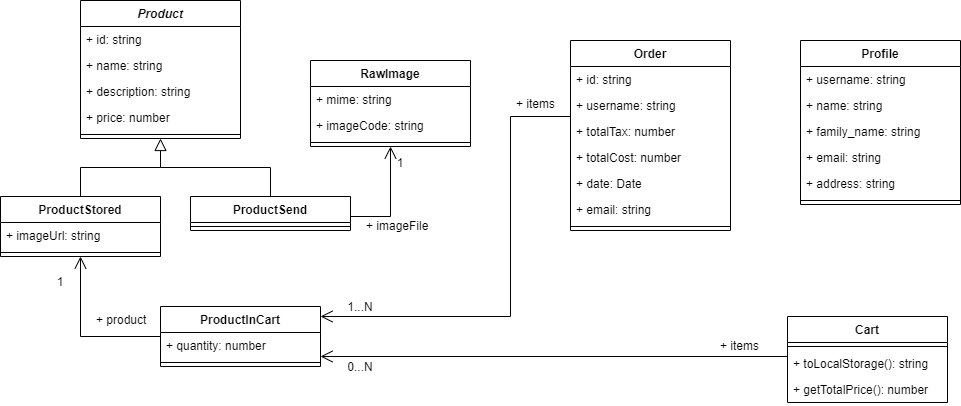
\includegraphics[scale=0.45]{res/Architettura/Frontend/img/class_frontend_types}\\
\caption{Diagramma delle classi dei tipi utilizzati per il modulo Front-end\ped{G}}
\end{figure}
\subsubsection{Diagrammi di sequenza}
Di seguito il diagramma di sequenza del modulo \textbf{Front-end\ped{G}} relativo all'inserimento di un prodotto nel carrello dalla pagina di listino prodotti.

\vspace{1cm}

\begin{figure}[H]
\centering
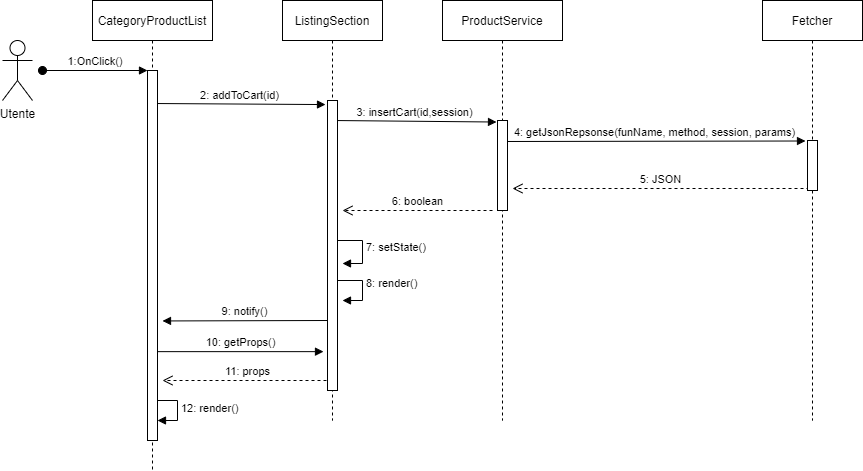
\includegraphics[scale=0.5]{res/Architettura/Frontend/img/sequence_frontend_insertCart}\\
\caption{Diagramma di sequenza dell'inserimento di un prodtto nel carrello del modulo Front-end\ped{G}}
\end{figure}

\newpage

\subsection{Architettura modulo Back-end}


\subsubsection{Descrizione}
In questo modulo, chiamato \textbf{Back-end\ped{G}}, viene gestita la logica interna del sito \nameproject. In particolare viene amministrato l'accesso al lato \textbf{business} dell'applicativo, e la parte relativa alla persistenza dei dati salvati all'interno dei servizi offerti da Amazon AWS\ped{G}. L'architettura generale del modulo è basata sui microservizi offerti dalle chiamate API, i quali hanno una base in comune sviluppata a \textbf{layer}, dove i tre layer principali sono:
\begin{itemize}
	\item \textbf{Handler\ped{G} delle API\ped{G}}: gestori delle richieste suddivise per dominio;
	\item \textbf{Model}: gestione logica dei modelli delle entità rappresentate (prodotto, utente...);
	\item \textbf{Services}: gestione dei servizi Amazon AWS\ped{G} e complementari.
\end{itemize} Il modulo \textbf{Front-end\ped{G}} interagisce con il modulo \textbf{Back-end\ped{G}} attraverso delle chiamate API\ped{G} esposte del servizio Amazon API Gateway. Tali API\ped{G} sono divise per dominio relativo all'oggetto con cui si vuole interagire e alla sua funzionalità (es. inserimento di un nuovo prodotto). L'handler\ped{G} gestisce la richiesta in base alla propria funzionalità e smista la relativa richiesta, dopo un opportuno controllo, sul \textbf{layer dei servizi} (dove necessario). I servizi offerti comprendono l'interfacciamento con DynamoDB, Stripe, S3, Nodemailer, Cognito. Inoltre, sempre dove necessario, l'handler\ped{G} della richiesta può interfacciarsi con il \textbf{layer dei modelli} degli oggetti (prodotto, utente ecc..) i quali forniranno supporto per la gestione logica di tali elementi.

\vspace{1cm}

\begin{figure}[H]
\centering
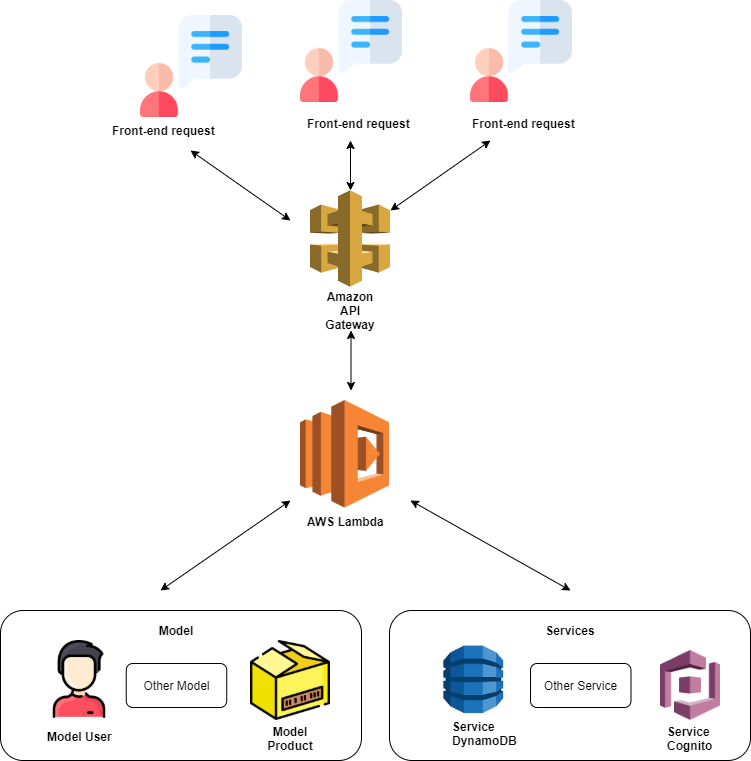
\includegraphics[scale=0.40]{res/Architettura/Backend/img/layerBack-end.png}\\
\caption{Layer del modulo Back-end\ped{G}}
\end{figure}
\subsubsection{Diagramma dei package}

Di seguito è riportato il diagramma dei package\ped{G} del modulo \textbf{Front-end\ped{G}}.

\vspace{1cm}

\begin{figure}[H]
\centering
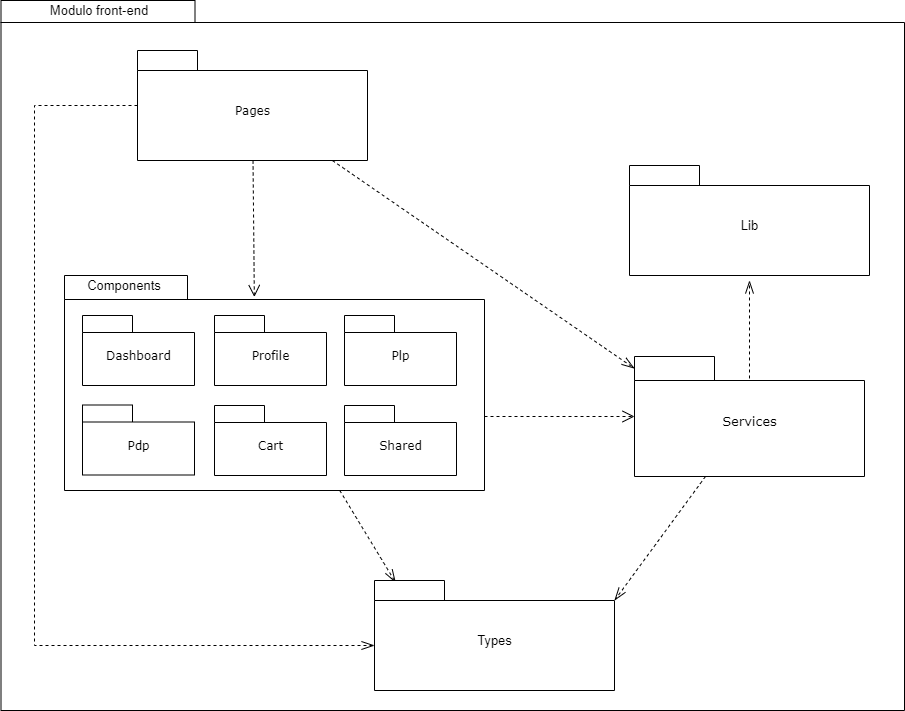
\includegraphics[scale=0.43]{res/Architettura/Frontend/img/package_frontend.png}\\
\caption{Diagramma dei package\ped{G} del modulo Front-end\ped{G}}
\end{figure}
\subsubsection{Diagramma delle classi}
Di seguito è riportato un esempio di diagramma delle classi. Esso rappresenta come è composta la pagina della dashboard\ped{G} e come vengono gestiti i vari component presentational e container.

\vspace{1cm}

\begin{figure}[H]
\centering
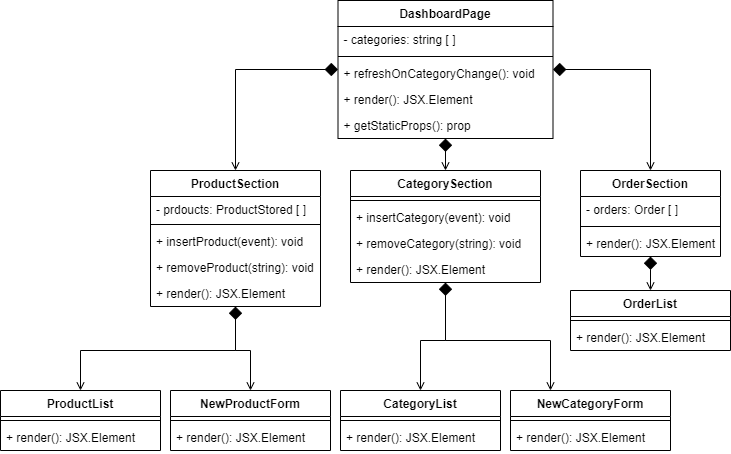
\includegraphics[scale=0.55]{res/Architettura/Frontend/img/class_frontend_dashboard}\\
\caption{Diagramma delle classi della pagina dashboard\ped{G} per il modulo Front-end\ped{G}}
\end{figure}

Viene inoltre mostrato il diagramma per i diversi tipi utilizzati dal nostro modulo.

\begin{figure}[H]
\centering
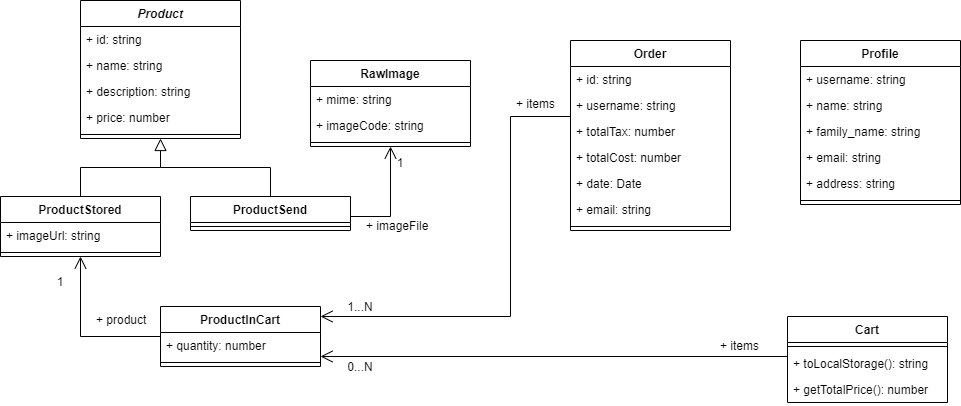
\includegraphics[scale=0.45]{res/Architettura/Frontend/img/class_frontend_types}\\
\caption{Diagramma delle classi dei tipi utilizzati per il modulo Front-end\ped{G}}
\end{figure}
\subsubsection{Diagrammi di sequenza}
Di seguito il diagramma di sequenza del modulo \textbf{Front-end\ped{G}} relativo all'inserimento di un prodotto nel carrello dalla pagina di listino prodotti.

\vspace{1cm}

\begin{figure}[H]
\centering
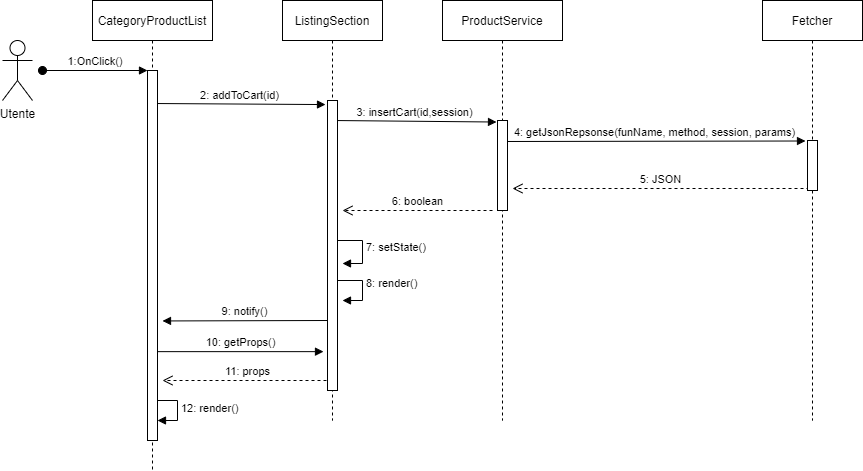
\includegraphics[scale=0.5]{res/Architettura/Frontend/img/sequence_frontend_insertCart}\\
\caption{Diagramma di sequenza dell'inserimento di un prodtto nel carrello del modulo Front-end\ped{G}}
\end{figure}

